\clearpage

\subsection{Conclusions}
\begin{tcolorbox}	
\begin{tabular}{p{2.75cm} p{0.2cm} p{10.5cm}} 	
\textbf{Student Name}  &:& Tiago Esteves    (October 03, 2017 - )\\
\textbf{Goal}          &:& Conclusions about the ILPs created and their results.
\end{tabular}
\end{tcolorbox}
\vspace{11pt}

After realizing the ILP models for the three transport modes we will focus on these results obtained and draw as many conclusions as possible from these results. For this, the graph xxxx is created with the information obtained previously.\\

\begin{center}
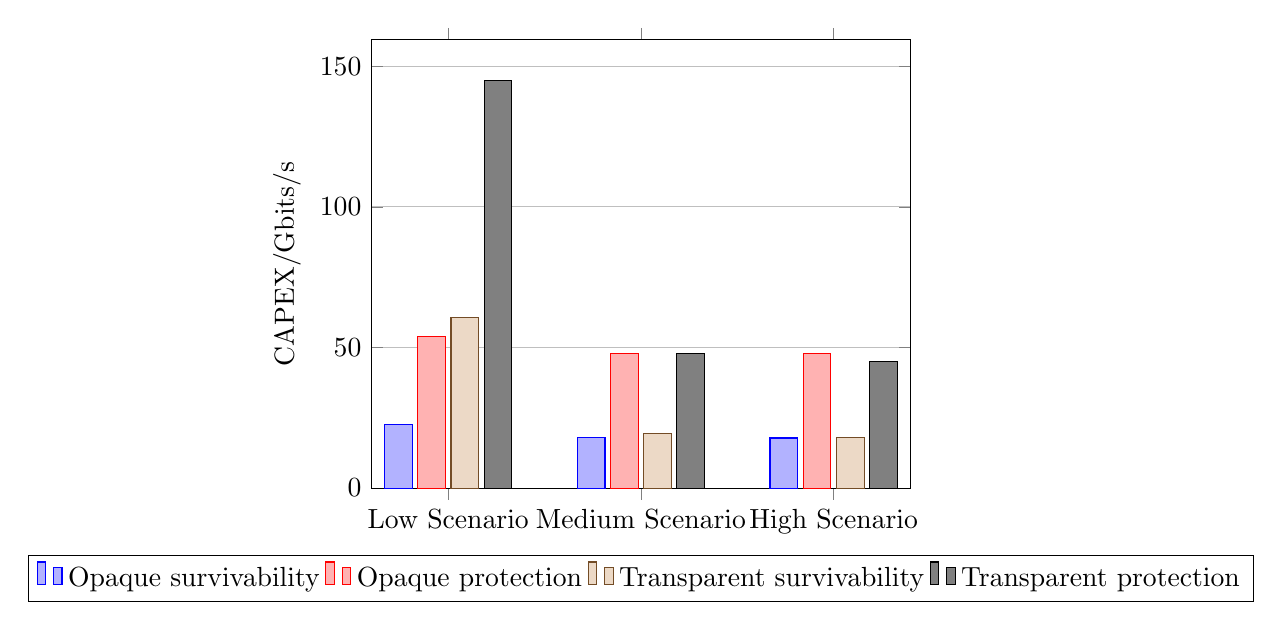
\begin{tikzpicture}
\begin{axis}[
ylabel=CAPEX/Gbits/s,
enlarge x limits=0.2,
legend style={
    at={(0.5,-0.15)},
    anchor=north,legend columns=-1
},
ymin=0,
ybar,
xtick=data,
symbolic x coords={Low Scenario,Medium Scenario,High Scenario},
grid=major,
xmajorgrids=false
]
\addplot coordinates {(Low Scenario,22.533) (Medium Scenario,18.121) (High Scenario,17.823)};
\addplot coordinates {(Low Scenario,53.965) (Medium Scenario,47.881) (High Scenario,47.703)};
\addplot coordinates {(Low Scenario,60.630) (Medium Scenario,19.366) (High Scenario,18.047)};
\addplot coordinates {(Low Scenario,144.935) (Medium Scenario,47.908) (High Scenario,44.880)};
\legend{Opaque survivability,Opaque protection,Transparent survivability,Transparent protection}
\end{axis}
\end{tikzpicture}
\end{center} 